% Detailed layer-level architecture of CrossAttentionFusion (figure 1b).
% AlexNet/GoogLeNet-style: every layer + tensor shape, with the repeated
% TransformerDecoderLayer expanded (D=512, T<=3 conditions, 4 heads, x2 layers).
% Build:  pdflatex architecture_detail.tex   then   pdftocairo -svg architecture_detail.pdf
\documentclass[border=8pt]{standalone}
% Shared TikZ palette + primitive styles for the paper-style schematics.
% \input-ed by architecture.tex and training.tex. Colours ported from the old
% figures/toolkit.py PALETTE / EDGE / BAND_TINT.
\usepackage{tikz}
\usepackage{amsmath,amssymb,bm}
\usetikzlibrary{arrows.meta,positioning,fit,backgrounds,shadows.blur,calc}

% --- palette ---------------------------------------------------------------
\definecolor{ink}{HTML}{2B2B35}
\definecolor{muted}{HTML}{6B6B78}
\definecolor{line}{HTML}{9AA0AD}

\definecolor{clipFill}{HTML}{DBE7F5}\definecolor{clipEdge}{HTML}{7FA8D4}\definecolor{clipTint}{HTML}{EEF4FB}
\definecolor{queryFill}{HTML}{F5E6CC}\definecolor{queryEdge}{HTML}{D8B878}\definecolor{queryTint}{HTML}{FBF4E6}
\definecolor{trainFill}{HTML}{CDEACD}\definecolor{trainEdge}{HTML}{85C285}\definecolor{trainTint}{HTML}{EEF7EE}
\definecolor{negFill}{HTML}{F3D6D6}\definecolor{negEdge}{HTML}{DD9B9B}\definecolor{negTint}{HTML}{FCEEEE}
\definecolor{fuseFill}{HTML}{E8D6F3}\definecolor{fuseEdge}{HTML}{C298D8}\definecolor{fuseTint}{HTML}{F6EEFB}

\definecolor{posFill}{HTML}{D9EFD9}\definecolor{posEdge}{HTML}{5FAE5F}\definecolor{posInk}{HTML}{235C23}
\definecolor{negPillFill}{HTML}{F6D9D9}\definecolor{negPillEdge}{HTML}{D98989}\definecolor{negPillInk}{HTML}{7A2B2B}
\definecolor{goodGreen}{HTML}{2E7D32}
\definecolor{badRed}{HTML}{B3322F}
\definecolor{frostBlue}{HTML}{3D7CC0}
\definecolor{emberOrange}{HTML}{E8772E}
\definecolor{biton}{HTML}{7FA8D4}
\definecolor{bitflip}{HTML}{E0A52E}
\definecolor{avatarTile}{HTML}{F3F1EE}
\definecolor{avatarSil}{HTML}{B9BCC4}
\definecolor{badgeOk}{HTML}{2E9E4F}
\definecolor{badgeNo}{HTML}{CF4F4F}

% --- base styles -----------------------------------------------------------
\tikzset{
  every node/.style={font=\sffamily,text=ink},
  >={Stealth[round]},
  % rounded panel with soft shadow; role colours set via fill=...Fill, draw=...Edge
  panel/.style={rounded corners=4pt,draw,line width=0.9pt,blur shadow={shadow blur steps=5,
                shadow xshift=1.2pt,shadow yshift=-1.2pt,shadow opacity=28}},
  clip/.style ={panel,fill=clipFill, draw=clipEdge},
  query/.style={panel,fill=queryFill,draw=queryEdge},
  train/.style={panel,fill=trainFill,draw=trainEdge},
  neg/.style  ={panel,fill=negFill,  draw=negEdge},
  fuse/.style ={panel,fill=fuseFill, draw=fuseEdge},
  % a titled block: #1 = role style; use \blk macro below for title+subtitle text
  blk/.style 2 args={#1,align=center,inner sep=5pt},
  % stage band: dashed tinted backdrop drawn on the background layer
  band/.style={rounded corners=6pt,draw,line width=0.8pt,dash pattern=on 4pt off 3pt,
               inner sep=10pt},
  bandclip/.style ={band,fill=clipTint, draw=clipEdge},
  bandquery/.style={band,fill=queryTint,draw=queryEdge},
  bandtrain/.style={band,fill=trainTint,draw=trainEdge},
  bandneg/.style  ={band,fill=negTint,  draw=negEdge},
  bandfuse/.style ={band,fill=fuseTint, draw=fuseEdge},
  % signed pills
  pillpos/.style={rounded corners=7pt,fill=posFill,draw=posEdge,line width=0.9pt,
                  text=posInk,font=\sffamily\bfseries\small,inner sep=4pt},
  pillneg/.style={rounded corners=7pt,fill=negPillFill,draw=negPillEdge,line width=0.9pt,
                  text=negPillInk,font=\sffamily\bfseries\small,inner sep=4pt},
  % wires
  wire/.style={->,line width=1.1pt,ink},
  skipwire/.style={->,line width=1.0pt,muted,dash pattern=on 4pt off 3pt},
  % attribute-grid cells
  bitoff/.style={draw=line,line width=0.6pt,fill=white,minimum size=6pt,inner sep=0pt},
  biton/.style ={draw=line,line width=0.6pt,fill=biton,minimum size=6pt,inner sep=0pt},
  bitflip/.style={draw=bitflip,line width=1.5pt,minimum size=6pt,inner sep=0pt},
  wiretag/.style={font=\sffamily\scriptsize,text=muted,fill=white,inner sep=1.5pt,
                  fill opacity=0.85,text opacity=1},
  % --- layer-level (AlexNet/GoogLeNet-style) primitives ---
  lyr/.style={rounded corners=3pt,draw,line width=0.9pt,align=center,inner sep=4pt,
              font=\sffamily\small,fill=white,minimum height=0.78cm,minimum width=2.2cm},
  clipL/.style ={lyr,fill=clipFill, draw=clipEdge},
  queryL/.style={lyr,fill=queryFill,draw=queryEdge},
  trainL/.style={lyr,fill=trainFill,draw=trainEdge},
  negL/.style  ={lyr,fill=negFill,  draw=negEdge},
  fuseL/.style ={lyr,fill=fuseFill, draw=fuseEdge},
  % small elementwise-op node (\opn{$\oplus$})
  opn/.style={circle,draw=ink,line width=0.8pt,inner sep=0.5pt,font=\footnotesize,
              fill=white,minimum size=0.42cm},
  flow/.style={->,line width=1.0pt,ink},
}
% shape tag appended under a layer title: Title\dm{(B, 512)}
\newcommand{\dm}[1]{\\[1.5pt]{\ttfamily\scriptsize\color{muted}#1}}

% titled block: \blkbox{name}{role}{x,y}{width}{Title}{subtitle}
\newcommand{\blkbox}[6]{%
  \node[#2,minimum width=#4,align=center,inner sep=4pt] (#1) at (#3)
       {{\bfseries\small #5}\\[1pt]{\scriptsize\color{muted}#6}};}

% legend swatch
\newcommand{\swatch}[2]{\tikz[baseline=-0.5ex]\node[rounded corners=2pt,fill=#1,
  minimum width=9pt,minimum height=9pt,inner sep=0pt]{};~{\scriptsize #2}}

% placeholder face thumbnail: \avatar{name}{cx}{cy}{half-size}{edge colour}
\newcommand{\avatar}[5]{%
  \draw[rounded corners=2.5pt,fill=avatarTile,draw=#5,line width=1.1pt]
       (#2-#4,#3-#4) rectangle (#2+#4,#3+#4);
  \coordinate (#1) at (#2,#3);
  \begin{scope}
    \clip[rounded corners=2.5pt] (#2-#4,#3-#4) rectangle (#2+#4,#3+#4);
    \fill[avatarSil] (#2,#3+0.30*#4) circle ({0.55*#4});
    \fill[avatarSil] (#2,#3-0.55*#4) ellipse ({0.95*#4} and {0.72*#4});
  \end{scope}}
% pass/fail badge on the top-right of an avatar: \badge{cx}{cy}{half-size}{ok|no}
\newcommand{\badge}[4]{%
  \edef\bcol{\ifnum\pdfstrcmp{#4}{ok}=0 badgeOk\else badgeNo\fi}%
  \edef\bsym{\ifnum\pdfstrcmp{#4}{ok}=0 \noexpand\checkmark\else $\noexpand\times$\fi}%
  \draw[fill=\bcol,draw=white,line width=1.2pt] (#1+0.7*#3,#2+0.7*#3) circle ({0.42*#3});
  \node[text=white,font=\sffamily\bfseries\tiny] at (#1+0.7*#3,#2+0.7*#3) {\bsym};}

% 24-bit attribute grid (8 cols): \bitgrid{x}{y}{bit-string}{flip-list}
% bit-string: comma list of 0/1 (length 24); flip-list: comma indices (1-based) drawn highlighted
\newcommand{\bitgrid}[4]{%
  \begin{scope}[shift={(#1,#2)}]
    \foreach \bv [count=\i from 0] in {#3} {%
      \pgfmathtruncatemacro{\row}{div(\i,8)}\pgfmathtruncatemacro{\col}{mod(\i,8)}%
      \ifnum\bv=1\relax
        \node[biton]  (bc\i) at (0.24*\col,-0.24*\row) {};%
      \else
        \node[bitoff] (bc\i) at (0.24*\col,-0.24*\row) {};%
      \fi}%
    \edef\tmpflip{#4}%
    \ifx\tmpflip\empty\else
      \foreach \f in {#4} {\pgfmathtruncatemacro{\j}{\f-1}\node[bitflip] at (bc\j) {};}%
    \fi
  \end{scope}}

\tikzset{
  lnb/.style={rounded corners=2pt,draw=line,line width=0.7pt,fill=black!4,
              font=\sffamily\scriptsize,inner sep=2.5pt,minimum width=2.2cm},
  note/.style={font=\sffamily\scriptsize,text=muted},
}
\begin{document}
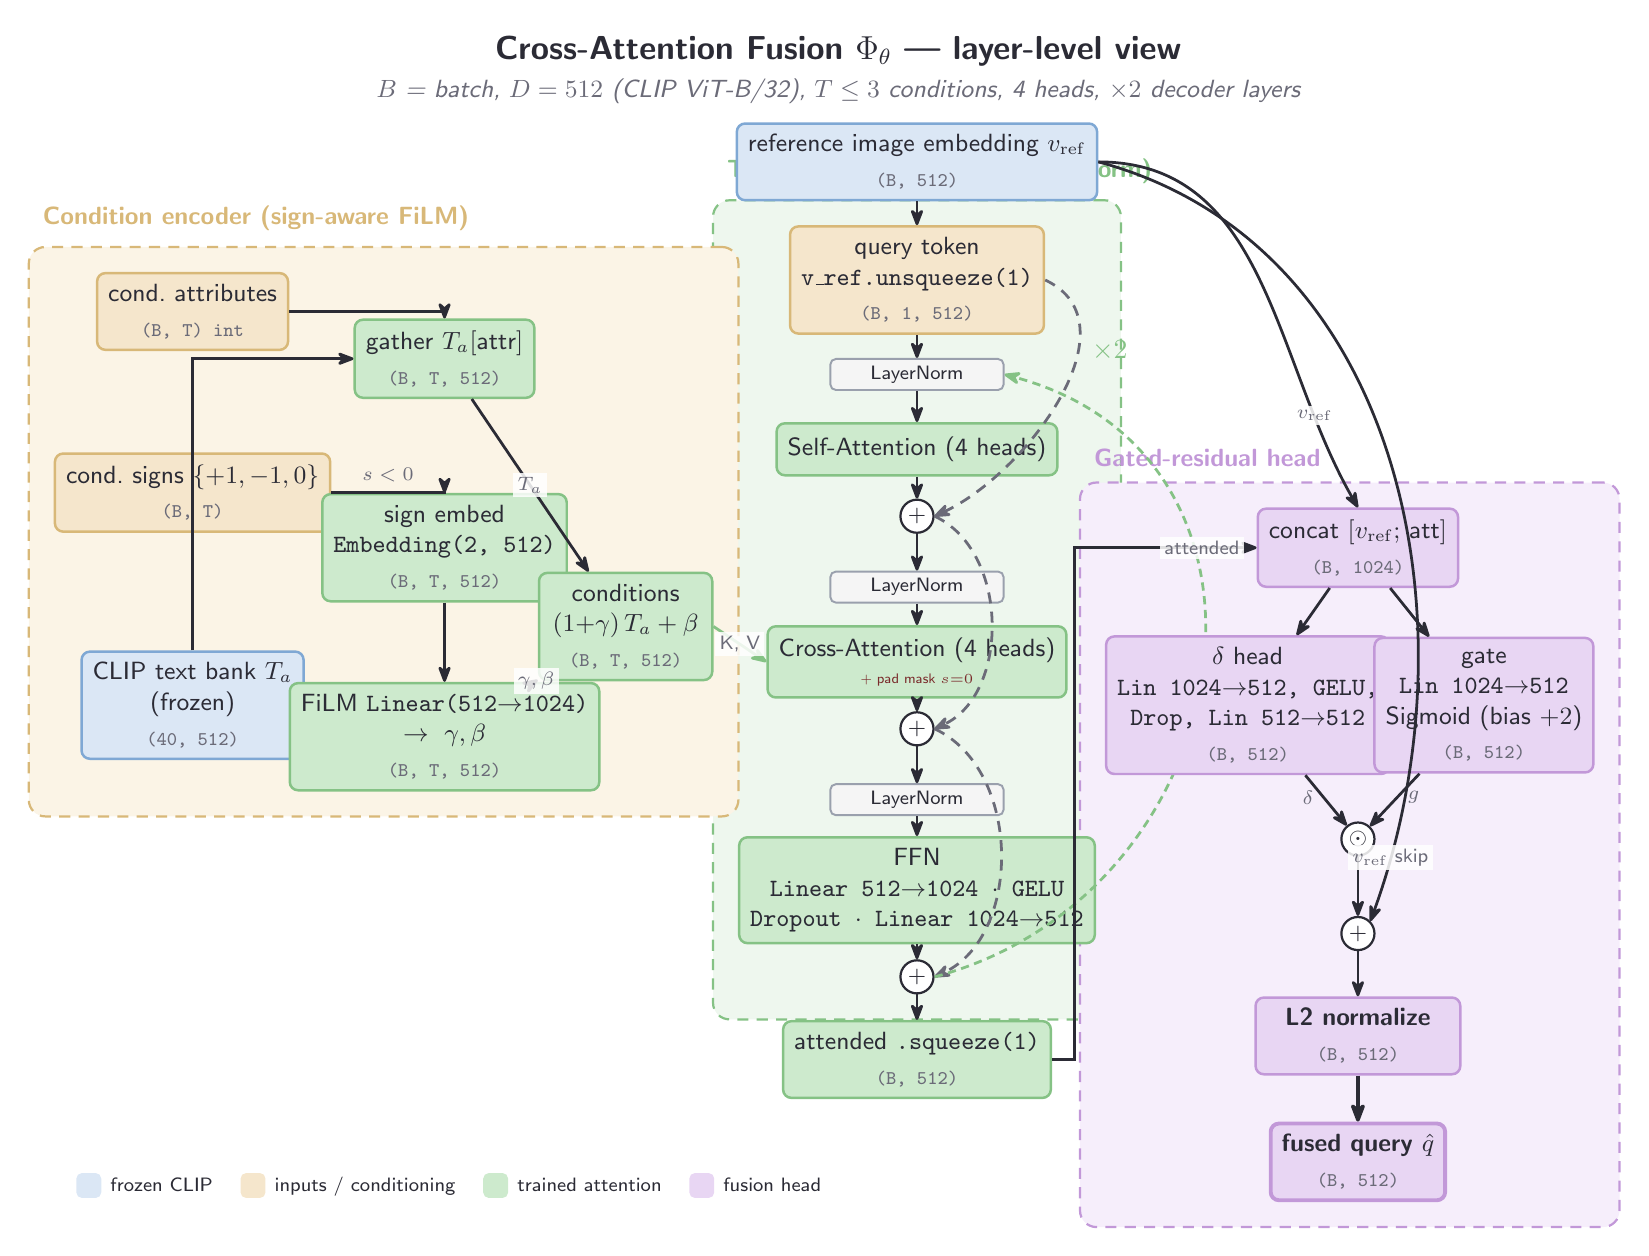
\begin{tikzpicture}[x=1cm,y=1cm]

  % ===== title =====
  \node[font=\sffamily\bfseries\large] at (10,13.5)
    {Cross-Attention Fusion $\Phi_\theta$ --- layer-level view};
  \node[note,font=\sffamily\itshape\small] at (10,13.0)
    {$B$ = batch, $D=512$ (CLIP ViT-B/32), $T\le3$ conditions, 4 heads, $\times2$ decoder layers};

  % ===== image input (top, feeds the query and the residual head) =====
  \node[clipL] (img) at (11.0,12.1) {reference image embedding $v_{\mathrm{ref}}$\dm{(B, 512)}};

  % ================= GROUP 1: condition encoder =================
  \node[queryL] (cattr) at (1.8,10.2) {cond.\ attributes\dm{(B, T) int}};
  \node[queryL] (csign) at (1.8,7.9)  {cond.\ signs $\{{+}1,{-}1,0\}$\dm{(B, T)}};
  \node[clipL]  (bank)  at (1.8,5.2)  {CLIP text bank $T_a$\\(frozen)\dm{(40, 512)}};

  \node[trainL] (gather) at (5.0,9.6) {gather $T_a[\text{attr}]$\dm{(B, T, 512)}};
  \node[trainL] (embed)  at (5.0,7.2) {sign embed\\\texttt{Embedding(2, 512)}\dm{(B, T, 512)}};
  \node[trainL] (film)   at (5.0,4.8) {FiLM \texttt{Linear(512$\to$1024)}\\$\to\ \gamma,\beta$\dm{(B, T, 512)}};
  \node[trainL] (conds)  at (7.3,6.2) {conditions\\$(1{+}\gamma)\,T_a+\beta$\dm{(B, T, 512)}};

  \draw[flow] (cattr) -| (gather);
  \draw[flow] (bank.north) |- (gather);
  \draw[flow] (csign) -| node[note,pos=0.25,above]{$s<0$} (embed);
  \draw[flow] (embed) -- (film);
  \draw[flow] (gather) -- node[wiretag,pos=0.5]{$T_a$} (conds);
  \draw[flow] (film) -- node[wiretag,pos=0.5]{$\gamma,\beta$} (conds);

  % ================= GROUP 2: cross-attention decoder (expanded) =================
  \def\cx{11.0}
  \node[queryL] (q)  at (\cx,10.6) {query token\\\texttt{v\_ref.unsqueeze(1)}\dm{(B, 1, 512)}};
  \node[lnb]    (ln1) at (\cx,9.4) {LayerNorm};
  \node[trainL,minimum height=0.66cm] (sa) at (\cx,8.45) {Self-Attention (4 heads)};
  \node[opn]    (a1) at (\cx,7.6) {$+$};
  \node[lnb]    (ln2) at (\cx,6.7) {LayerNorm};
  \node[trainL,minimum height=0.66cm] (ca) at (\cx,5.75)
        {Cross-Attention (4 heads)\\[-1pt]{\tiny\color{negPillInk}+ pad mask $s{=}0$}};
  \node[opn]    (a2) at (\cx,4.9) {$+$};
  \node[lnb]    (ln3) at (\cx,4.0) {LayerNorm};
  \node[trainL,minimum height=1.0cm] (ffn) at (\cx,2.85)
        {FFN\\\texttt{Linear 512$\to$1024 $\cdot$ GELU}\\\texttt{Dropout $\cdot$ Linear 1024$\to$512}};
  \node[opn]    (a3) at (\cx,1.75) {$+$};
  \node[trainL] (att) at (\cx,0.7) {attended\ \texttt{.squeeze(1)}\dm{(B, 512)}};

  \draw[flow] (img) -- (q);
  \draw[flow] (q) -- (ln1);  \draw[flow] (ln1) -- (sa);  \draw[flow] (sa) -- (a1);
  \draw[flow] (a1) -- (ln2); \draw[flow] (ln2) -- (ca);  \draw[flow] (ca) -- (a2);
  \draw[flow] (a2) -- (ln3); \draw[flow] (ln3) -- (ffn); \draw[flow] (ffn) -- (a3);
  \draw[flow] (a3) -- (att);
  % residual skips, bowing to the right
  \draw[skipwire] (q.east)  to[out=-25,in=25] (a1.east);
  \draw[skipwire] (a1.east) to[out=-25,in=25] (a2.east);
  \draw[skipwire] (a2.east) to[out=-25,in=25] (a3.east);
  % conditions -> K,V of cross-attention
  \draw[flow,trainEdge] (conds.east) -- node[wiretag,pos=0.5]{K, V} (ca.west);

  % decoder container + x2
  \begin{scope}[on background layer]
    \node[bandtrain,fit=(q)(ln1)(sa)(a1)(ca)(a2)(ffn)(a3),inner sep=9pt,
          label={[anchor=south west,font=\sffamily\bfseries\small,text=trainEdge,xshift=2pt,yshift=2pt]north west:TransformerDecoderLayer (pre-norm)}] (decbox) {};
  \end{scope}
  \node[trainEdge,font=\sffamily\bfseries] at (\cx+2.45,9.7) {$\times2$};
  \draw[->,trainEdge,line width=1pt,dash pattern=on 3pt off 2pt]
        (a3.east) to[out=15,in=-15,looseness=1.35]
        node[note,text=trainEdge,right,pos=0.5]{stack $\times2$} (ln1.east);

  % ================= GROUP 3: gated residual head =================
  \node[fuseL] (cat)   at (16.6,7.2) {concat $[v_{\mathrm{ref}};\,\text{att}]$\dm{(B, 1024)}};
  \node[fuseL] (delta) at (15.2,5.2) {$\delta$ head\\\texttt{Lin 1024$\to$512, GELU,}\\\texttt{Drop, Lin 512$\to$512}\dm{(B, 512)}};
  \node[fuseL] (gate)  at (18.2,5.2) {gate\\\texttt{Lin 1024$\to$512}\\Sigmoid (bias ${+}2$)\dm{(B, 512)}};
  \node[opn]   (mul)   at (16.6,3.5) {$\odot$};
  \node[opn]   (add)   at (16.6,2.3) {$+$};
  \node[fuseL,minimum width=2.6cm] (norm) at (16.6,1.0) {\textbf{L2 normalize}\dm{(B, 512)}};
  \node[fuseL,line width=1.4pt] (out) at (16.6,-0.6) {\textbf{fused query} $\hat q$\dm{(B, 512)}};

  \draw[flow] (att.east) -- (13.0,0.7) |- node[wiretag,pos=0.85]{attended} (cat.west);
  \draw[flow] (img.east) to[out=0,in=120] node[wiretag,pos=0.8]{$v_{\mathrm{ref}}$} (cat.north);
  \draw[flow] (cat) -- (delta);
  \draw[flow] (cat) -- (gate);
  \draw[flow] (delta) -- node[note,pos=0.45,left]{$\delta$} (mul);
  \draw[flow] (gate)  -- node[note,pos=0.45,right]{$g$} (mul);
  \draw[flow] (mul) -- (add);
  \draw[flow] (img.east) to[out=-15,in=70] node[wiretag,pos=0.93]{$v_{\mathrm{ref}}$ skip} (add.north east);
  \draw[flow] (add) -- (norm);
  \draw[flow,line width=1.3pt] (norm) -- (out);

  \begin{scope}[on background layer]
    \node[bandfuse,fit=(cat)(delta)(gate)(mul)(add)(norm)(out),inner sep=9pt,
          label={[anchor=south west,font=\sffamily\bfseries\small,text=fuseEdge,xshift=2pt,yshift=2pt]north west:Gated-residual head}] {};
    \node[bandquery,fit=(cattr)(csign)(bank)(gather)(embed)(film)(conds),inner sep=9pt,
          label={[anchor=south west,font=\sffamily\bfseries\small,text=queryEdge,xshift=2pt,yshift=2pt]north west:Condition encoder (sign-aware FiLM)}] {};
  \end{scope}

  % ===== legend =====
  \node[anchor=west,align=left,font=\sffamily] at (0.2,-0.9)
    {\swatch{clipFill}{frozen CLIP}\quad\swatch{queryFill}{inputs / conditioning}\quad
     \swatch{trainFill}{trained attention}\quad\swatch{fuseFill}{fusion head}};

\end{tikzpicture}
\end{document}
